\documentclass[12pt]{article}
\usepackage{geometry}
\geometry{left=2.5cm, right=2.5cm, top=2.5cm, bottom=2.5cm}
\usepackage{fancyhdr}
\pagestyle{fancy}
\fancyhead{} % 清空页眉
\fancyhead[C]{Fall 2024\hspace{3cm}CS430 Algorithm Introduction Project\hspace{3cm}		\thepage} % [C] 表示居中,也可以使用 L(左对齐)和 R(右对齐)
\fancyfoot{} % 清空页脚
\fancyfoot[C]{\thepage}
\usepackage{spverbatim}
\usepackage[english]{babel}
\usepackage{ctex}
\usepackage{amsmath}          % 数学公式包
\usepackage{graphicx}         % 图片包
\usepackage{caption}          % 标题包
\usepackage{subcaption}       % 子标题包
\usepackage{booktabs}         % 表格优化
\usepackage{hyperref}         % 超链接包
\usepackage{setspace}         % 设置行距包
\hypersetup{hidelinks}       % 去除链接的边框
\usepackage{times}
\usepackage{tcolorbox}
\usepackage{listings}
% 设置行距为1.5倍
\onehalfspacing

\title{Introduction to Algorithm \\ Project Report}  % 文档标题
\author{Liner Zhang}   % 作者姓名
\date{\today}          % 当前日期

\begin{document}

% 自定义封面
\begin{titlepage}
    \centering
    \vfill
    \Huge \textbf{Introduction to Algorithm} \\[0.5cm]  % 标题
    \Huge \textbf{Project Report} \\[10.0cm]  % 标题
    \Large Member: Liner Zhang \\[0.5cm]
    \Large CUG No: 20231003496  \\[0.5cm]
    \Large IIT No: A20563408 \\[0.5cm]
    \Large Teacher: Mr. Peng \\[0.5cm]
    \Large Date: December 16, 2024 \\[2.0cm]
\end{titlepage}

\tableofcontents  % 自动生成目录
\newpage

\section{Description of the Project} 
\subsection{Program Instruction}
Users simply need to fill in the "MyOriginalText.txt" file and click the "Run" button. The program will automatically generate the optimal Huffman encoding method, output the parameters $k$ and $n$, and calculate the shortest length of the encoded code. It will then save the results in several files: the Huffman dictionary will be saved to "MyCodeWorkBk.txt", the encoded text will be saved to "MyEncodingFile.txt", and the decoded text will be saved to "MyDecodingFile.txt". Additionally, the program will generate the Huffman tree in two formats: as text in "MyHuffmanFile.txt" and as an image in "MyHuffmanTree.png".

\subsection{Program Demonstration}
I provide a piece of material from \textit{Pride and Prejudice}, which contains over 3000 words. The contents of the file "MyOriginalText.txt" are shown in Figure 1.
\begin{figure}[htbp]
    \centering
    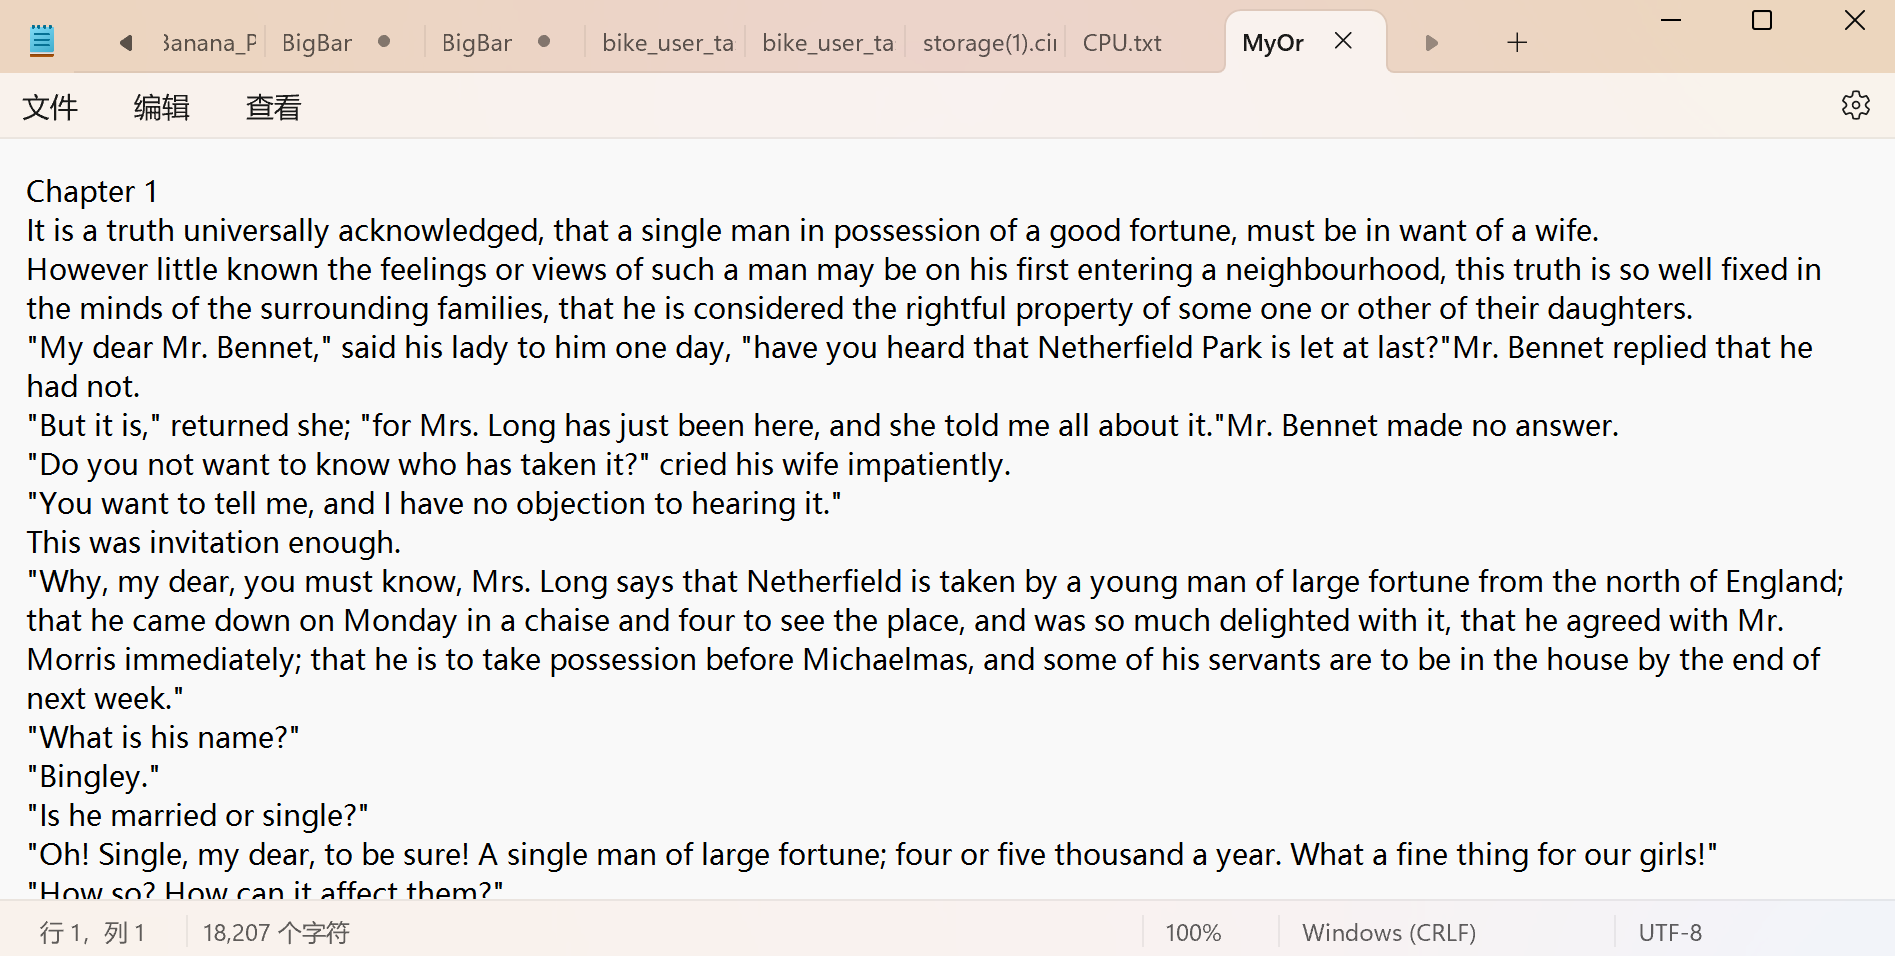
\includegraphics[width=0.9\textwidth]{input.png}
    \caption{MyOriginalText.txt}
    \label{pic1}
\end{figure}
\par The output of the program, representing the best-case result, along with the other related output files, is shown in Figures 2-7.
\par From Figure 2, we can determine that the shortest length of the encoded code is 73,879, which occurs when the top forty-five most frequent five-letter words are added to the Huffman tree.
\par From Figure 5, we can indeed identify several five-letter words.
\par From Figure 7, we can see the decoded text is the same as the origional text, which means the Huffman encoding method is effective.
\begin{figure}[htbp]
    \centering
    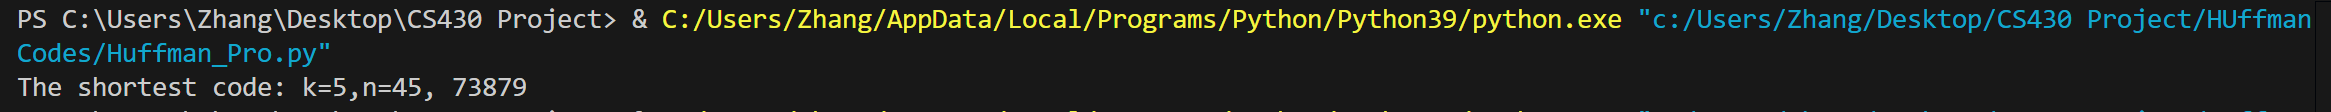
\includegraphics[width=\textwidth]{output.png}
    \caption{Program Output}
    \label{pic2}
\end{figure}

\begin{figure}[htbp]
    \centering
    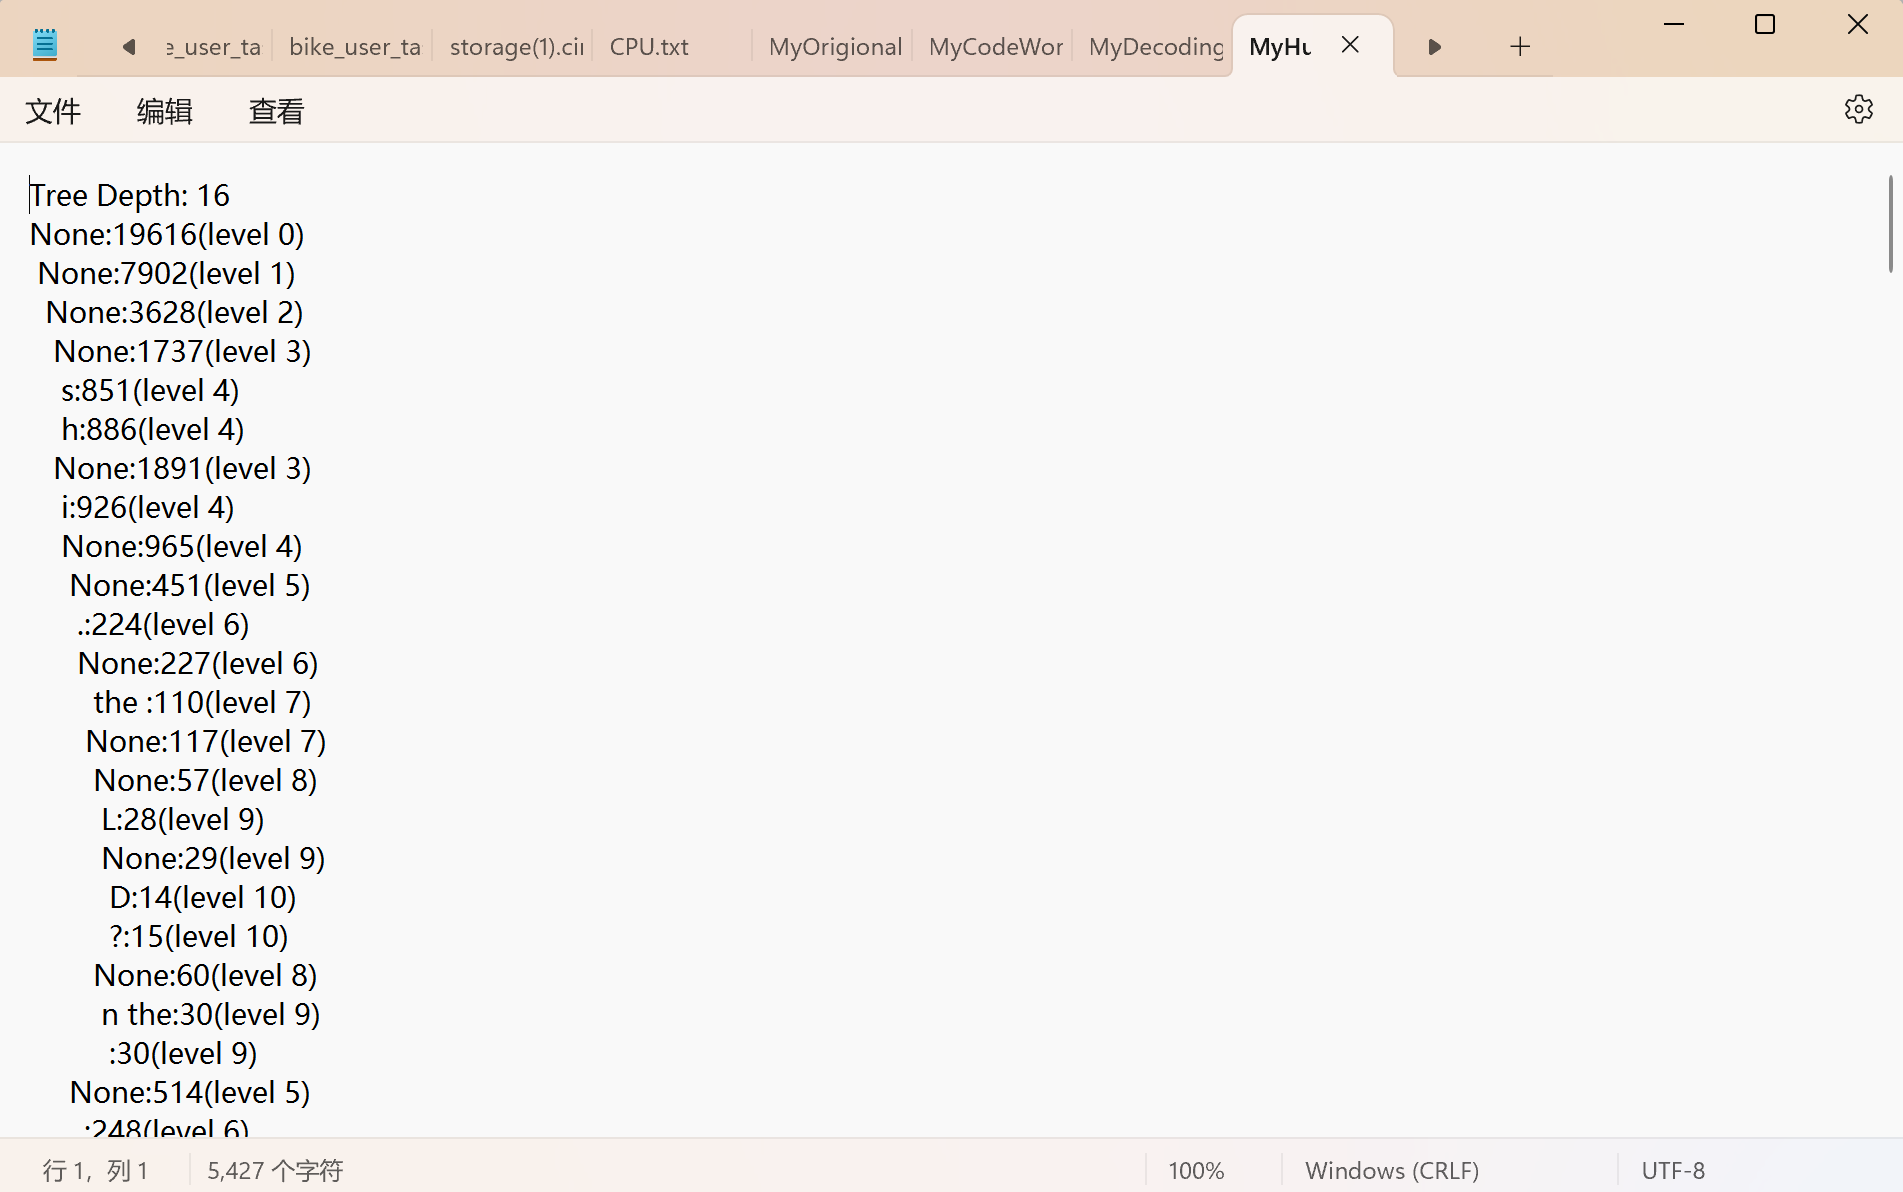
\includegraphics[width=0.9\textwidth]{tree.png}
    \caption{MyHuffmanFile.txt}
    \label{pic3}
\end{figure}

\begin{figure}[htbp]
    \centering
    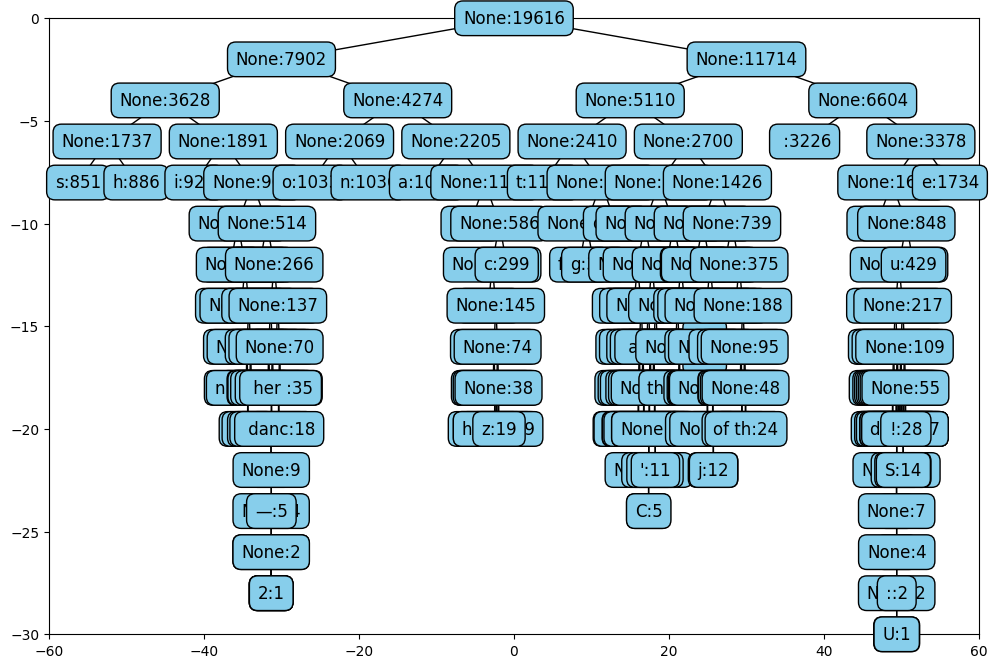
\includegraphics[width=0.9\textwidth]{MyHuffmanTree.png}
    \caption{MyHuffmanTree.png}
    \label{pic4}
\end{figure}

\begin{figure}[htbp]
    \centering
    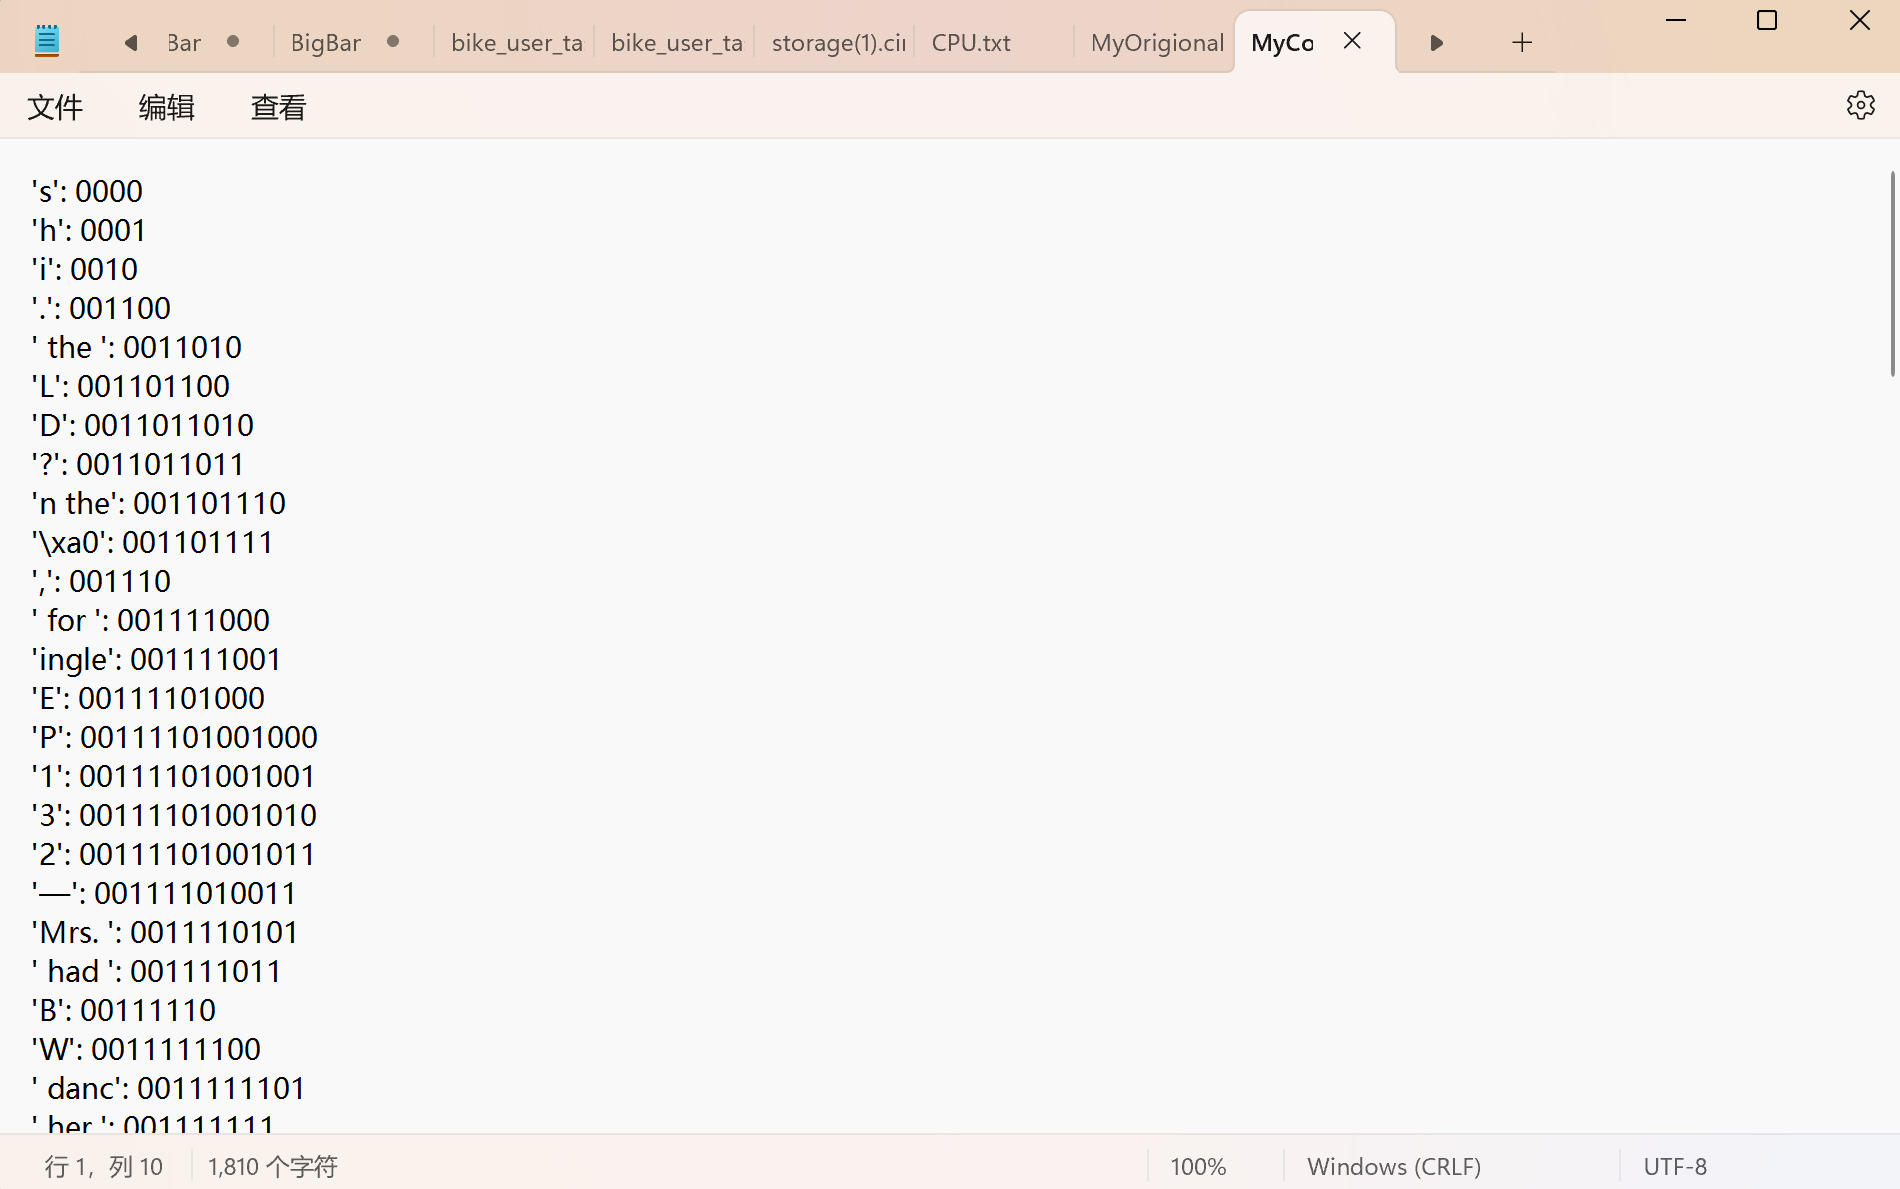
\includegraphics[width=0.9\textwidth]{dic.png}
    \caption{MyCodeWorkBk.txt}
    \label{pic5}
\end{figure}

\begin{figure}[htbp]
    \centering
    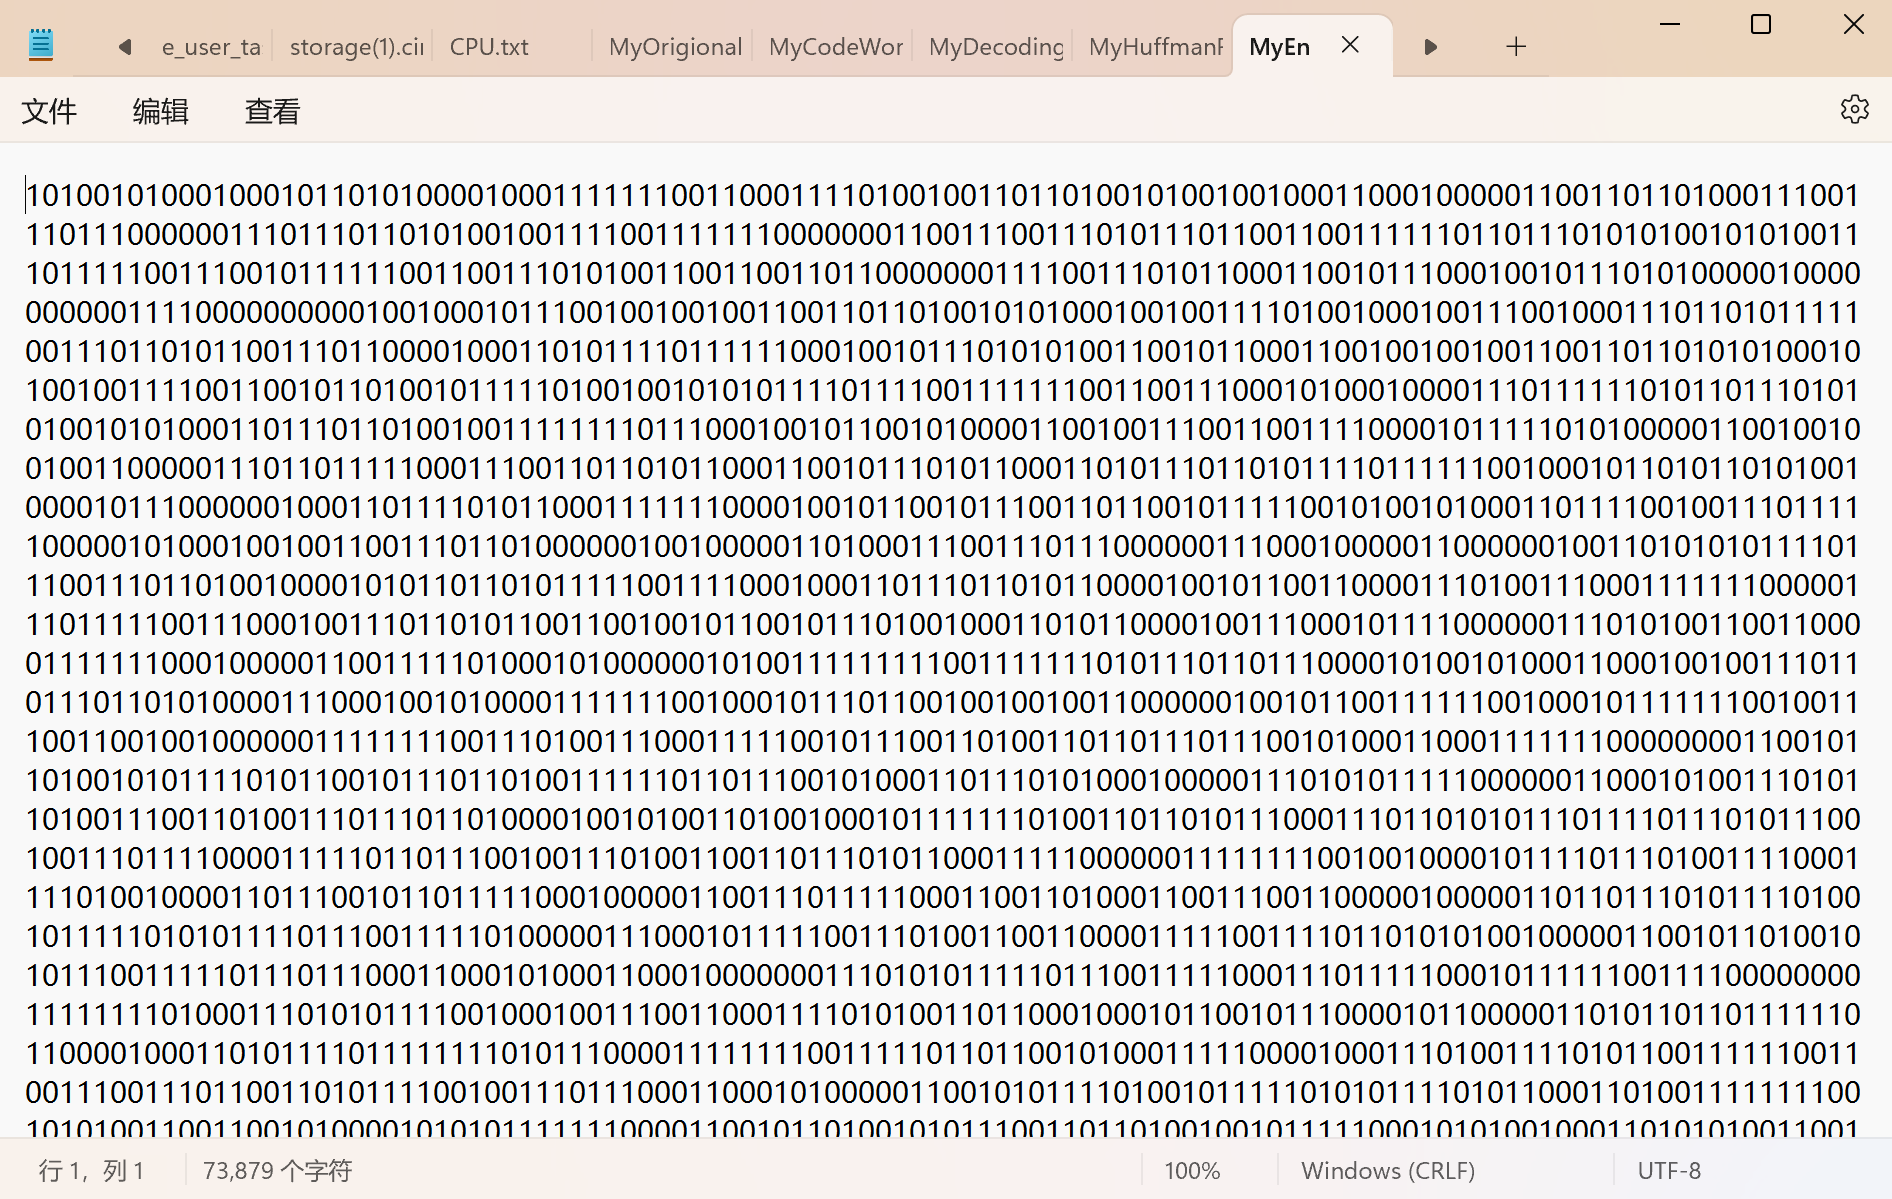
\includegraphics[width=0.9\textwidth]{encode.png}
    \caption{MyEncodingFile.txt}
    \label{pic6}
\end{figure}

\begin{figure}[htbp]
    \centering
    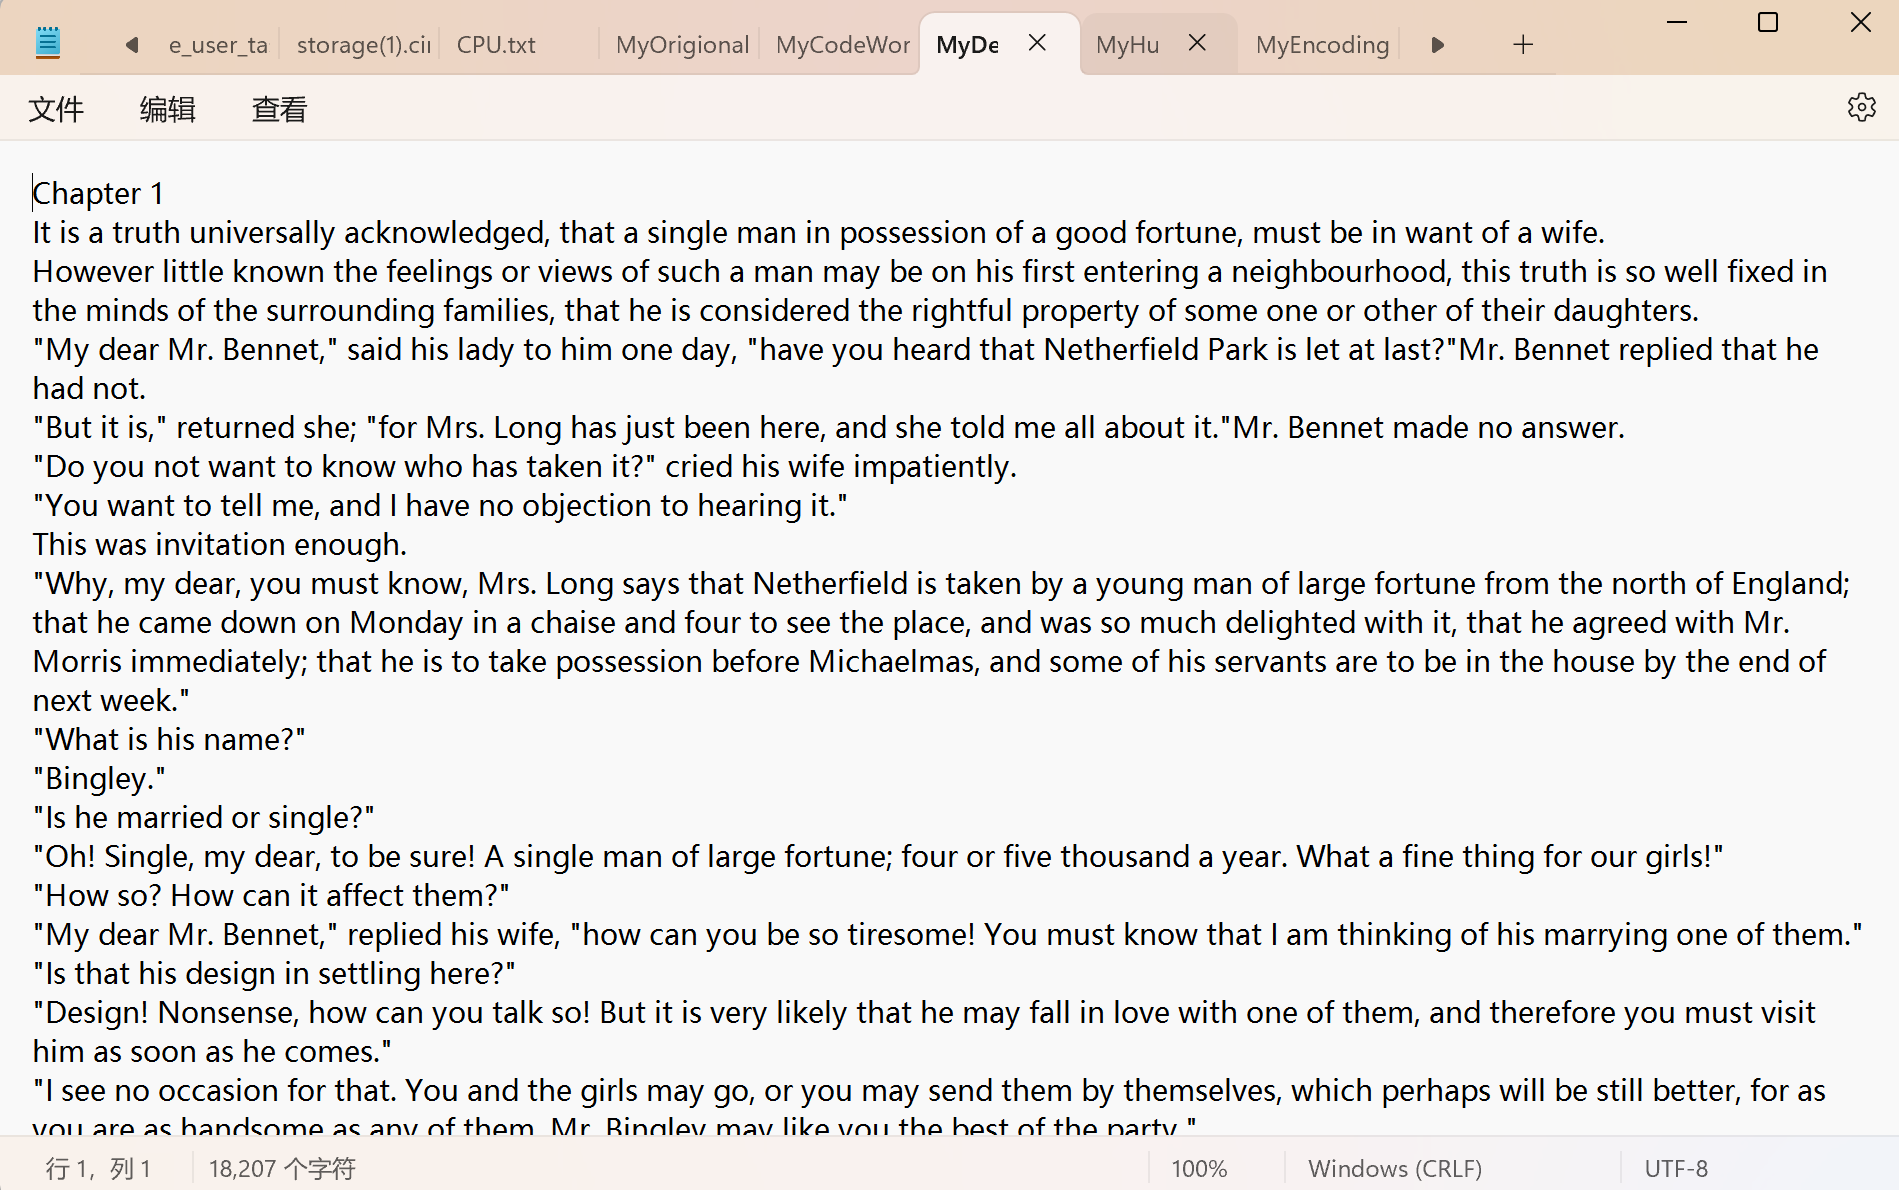
\includegraphics[width=0.9\textwidth]{decode.png}
    \caption{MyDecodingFile.txt}
    \label{pic7}
\end{figure}

\newpage
\section{Algorithm Design}
\par In designing the algorithm, I used the classic binary tree method to implement Huffman encoding. However, in addition to counting the frequency of individual letters, I also considered combinations of letters. To determine how many letter combinations to include and how many of the most frequent combinations to consider, I set two parameters to iterate and compare, in order to identify the parameter combination that produces the shortest encoded length. The detailed algorithm and code are as follows.
\begin{figure}[htbp]
    \centering
    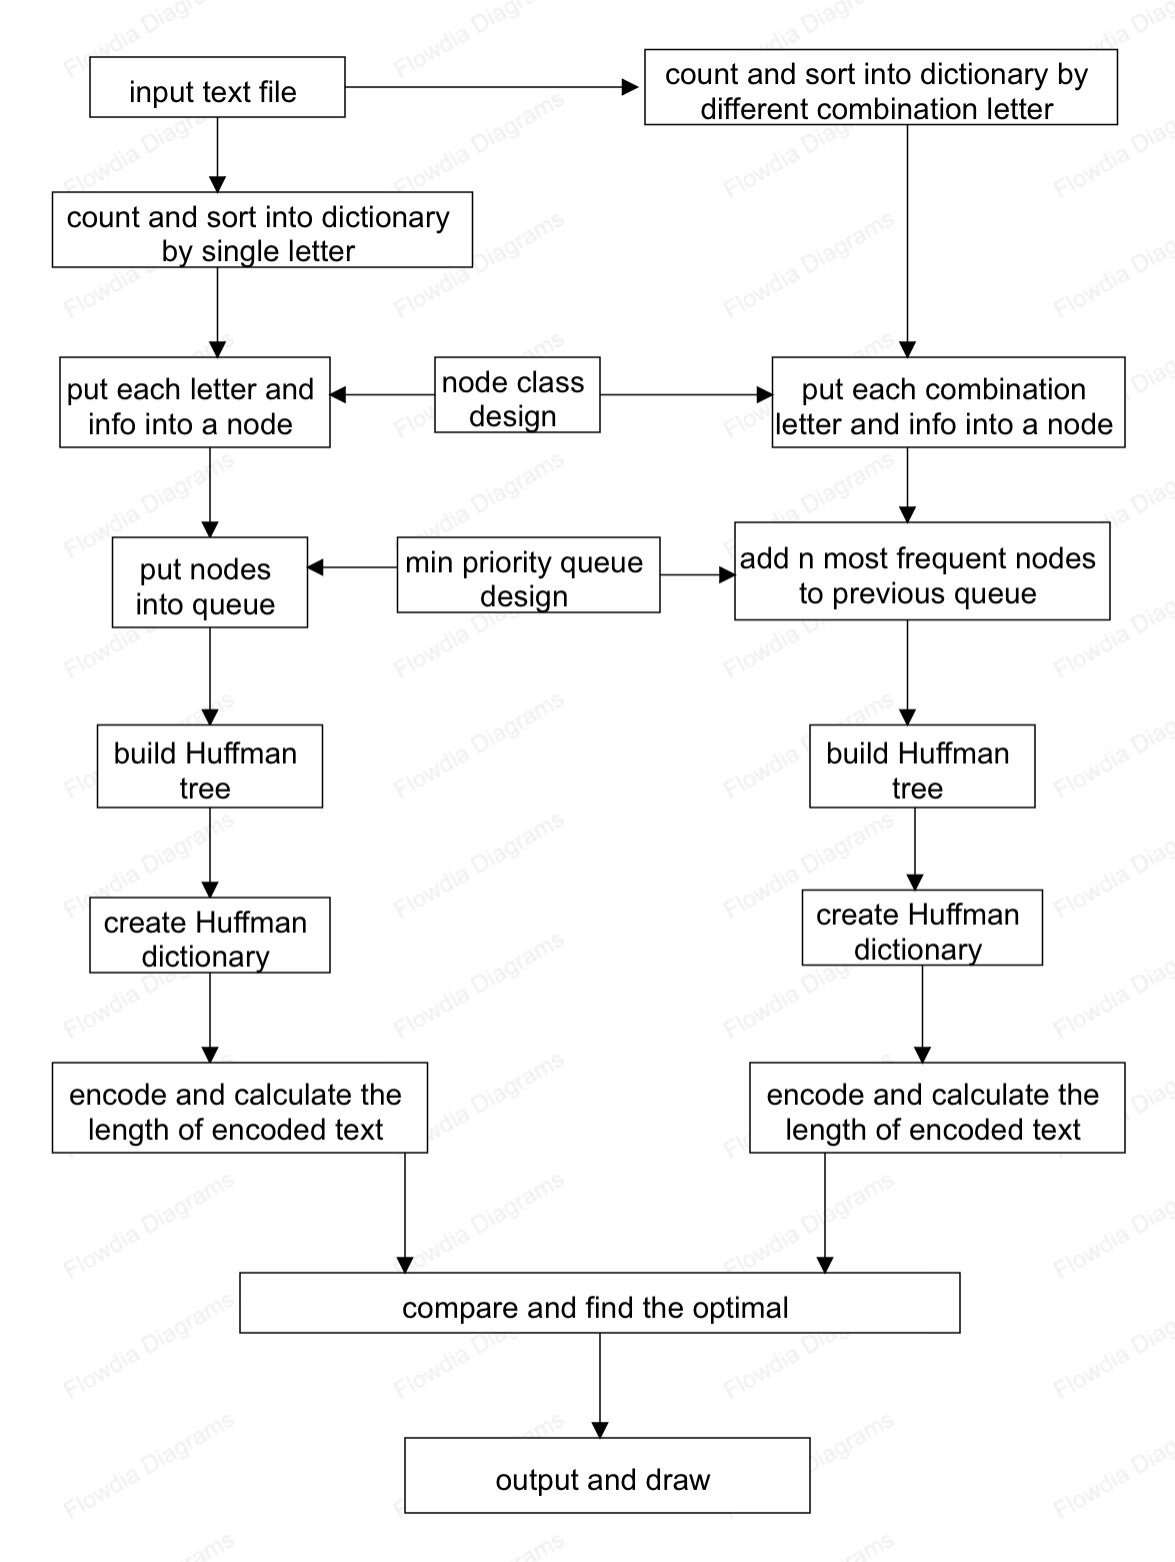
\includegraphics[width=0.7\textwidth]{flowchart.png}
    \caption{Flowchart}
    \label{pic8}
\end{figure}
\subsection{Data Processing}
\par Before starting the algorithm, the input document needs to be processed. First, the content of the document must be read and stored as a string. 
\par Based on my requirements, I also need to calculate the frequency of individual letters as well as the frequency of letter combinations, where k represents the number of letters in the combination. Since I will later need to map each letter to its corresponding frequency, I use a dictionary to store this mapping.
\begin{tcolorbox}[colframe=black, colback=white, boxrule=0.4mm, sharp corners=southwest, title=Data Processing Code]
\begin{lstlisting}[language=Python, breaklines=true]
def parse_file(input_file):
    with open(input_file, 'r', encoding='utf-8') as f:
        file = f.read() 
    return file
def count(file):
    counts = defaultdict(int)   
    for i in range(len(file)):
        counts[file[i]] += 1
    sorted_counts = sorted(counts.items(), key=lambda x: x[1], reverse=True)
    return sorted_counts
def count_1(file, k):
    counts_three = defaultdict(int)  
    for i in range(len(file)):
        if i + k - 1 < len(file): 
            counts_three[file[i:i+k]] += 1
    sorted_3 = sorted(counts_three.items(), key=lambda x: x[1], reverse=True)
    return sorted_3
\end{lstlisting}
\end{tcolorbox}
\subsection{Huffman Tree Construction}
Considering the algorithm, which requires continuously extracting the characters (or character combinations) with the least frequency and adding their frequencies together, a minimum queue is used here. In the queue class, it is specified that each time a new element is added, it should be placed in the correct position to ensure the elements in the queue are always sorted in descending order, and that the extracted element is always the minimum value. 
\par Additionally, since a tree needs to be built later, a Node class is designed to define the parent-child relationships and to store information associated with each node.
\par When constructing the Huffman tree, all characters (or character combinations) involved in the encoding are first placed into the queue. The add\_to\_tree function is then used to repeatedly extract the elements with the smallest frequencies, merge them, establish parent-child relationships, and put the merged elements back into the queue. This process continues until only one element remains in the queue, which becomes the root of the tree.
\begin{tcolorbox}[colframe=black, colback=white, boxrule=0.4mm, sharp corners=southwest, title=Queue Class Code]
    \begin{lstlisting}[language=Python, breaklines=true]
class min_queue:
    def __init__(self):
        self.queue=[]
    def enqueue(self, node):
        if not self.queue:
            self.queue.append(node)
        else:
            i = 0
            while i < len(self.queue) and self.queue[i].get_value() >= node.get_value():
                i += 1
            self.queue.insert(i, node)
    def dequeue(self):
        return self.queue.pop(-1)
    def length(self):
        return len(self.queue)
\end{lstlisting}
\end{tcolorbox}

\begin{tcolorbox}[colframe=black, colback=white, boxrule=0.4mm, sharp corners=southwest, title=Node Class Code]
    \begin{lstlisting}[language=Python, breaklines=true]
class Node:
    def __init__(self,char,value):
        self.char=char
        self.value=value
        self.left=None
        self.right=None
        self.code=None
        self.parent=None
    def __lt__(self, other):
        return self.value < other.value
    def left_child(self,node):
        self.left=node
    def right_child(self,node):
        self.right=node
    def set_parent(self,node):
        self.parent=node
    def get_left(self):
        return self.left
    def get_right(self):
        return self.right
    def get_parent(self):
        return self.parent
    def get_value(self):
        return self.value
    def get_char(self):
        return self.char
    def set_code(self,code):
        self.code=code
\end{lstlisting}
\end{tcolorbox}

\begin{tcolorbox}[colframe=black, colback=white, boxrule=0.4mm, sharp corners=southwest, title=Huffman Tree Construction Code]
    \begin{lstlisting}[language=Python, breaklines=true]
def add_to_tree(queue):
    if queue.length()==1:
        root=queue.dequeue()
        return root
    else:
        node1=queue.dequeue()
        node2=queue.dequeue()
        new_node=Node(None,node1.get_value()+node2.get_value())
        new_node.left_child(node1)
        new_node.right_child(node2)
        node1.set_parent(new_node)
        node2.set_parent(new_node)
        queue.enqueue(new_node)
        return add_to_tree(queue) 
        #add return !!!!!!!the problem is here!!!!!
def HuffmanTree_1(sorted_counts):
    queue=min_queue()
    for char,freq in sorted_counts:
        queue.enqueue(Node(char,freq))
    return add_to_tree(queue)
def HuffmanTree_2(sorted_counts,sorted_3,n):
    queue=min_queue()
    for char,freq in sorted_counts:
        queue.enqueue(Node(char,freq))
    for i in range(n):
        queue.enqueue(Node(sorted_3[i][0],sorted_3[i][1]))
    return add_to_tree(queue)
\end{lstlisting}
\end{tcolorbox}
\subsection{Huffman Dict Construction}
\par After obtaining the Huffman tree, the next step is to find the corresponding encoding for each leaf by traversing the tree. A depth-first search (DFS) approach, similar to left-child-first, is used. The add\_to\_tree function is repeatedly called to explore the tree from top to bottom and from left to right. When traversing, a 0 is added to the encoding for a left child, and a 1 is added for a right child. This process continues until a node's left and right children are both NIL, indicating it is a leaf node. The traversal then backtracks layer by layer, eventually determining the encoding for each leaf.
\begin{tcolorbox}[colframe=black, colback=white, boxrule=0.4mm, sharp corners=southwest, title=Huffman Dict Construction Code]
    \begin{lstlisting}[language=Python, breaklines=true]
def find_leaf(node, code,HuffDict):
    if node is None:
        return HuffDict#{char:code}
    if node.get_left() is None and node.get_right() is None: # It's a leaf node
        HuffDict[node.get_char()] = code
        return HuffDict
    if node.get_left() is not None:
        HuffDict = find_leaf(node.get_left(), code + "0", HuffDict)#until found the lefest node
    if node.get_right() is not None:
        HuffDict = find_leaf(node.get_right(), code + "1", HuffDict)
    return HuffDict      
def HuffmanDict(root):
    node=root
    HuffDict={}
    HuffDict=find_leaf(node,"",HuffDict)
    return HuffDict  
\end{lstlisting}
\end{tcolorbox}

\subsection{Huffman Encoding}
After obtaining the Huffman dictionary, the text can be encoded by matching each character with its corresponding entry in the dictionary. For character combinations, the next \( k \) characters in the text are checked to see if they exist as keys in the dictionary, and they are then encoded accordingly.
\begin{tcolorbox}[colframe=black, colback=white, boxrule=0.4mm, sharp corners=southwest, title=Huffman Encoding Code]
    \begin{lstlisting}[language=Python, breaklines=true]
def encode(file,HuffDict,k):
    encoded_text=""
    i=0
    while i<len(file):
        if file[i:i+k] in HuffDict:
            char=file[i:i+k]
            i+=k
        else:
            char=file[i]
            i+=1
        encoded_text+=HuffDict[char]
    return encoded_text
\end{lstlisting}
\end{tcolorbox}

\subsection{Optimal Huffman Solution}
After refining the encoding process, the next step is to compare encoding lengths for different parameters in order to find the optimal solution. The Huffman tree for individual characters is used as a baseline, with its encoding length denoted as \( l_1 \), which is considered the shortest encoding by default. For different values of \( k \) (i.e., different combinations of characters), the top \( n \)-frequent substrings are added to the single-character Huffman tree to generate new encodings. All relevant information for each parameter is stored in the info dictionary for later use. By continuously comparing the lengths of encodings generated with different parameters to the shortest encoding length, the optimal encoding method is identified, and all related information is returned.
\begin{tcolorbox}[colframe=black, colback=white, boxrule=0.4mm, sharp corners=southwest, title=Optimal Solution Code]
    \begin{lstlisting}[language=Python, breaklines=true]
def compare(file):
    ZLE=1   
    sorted_counts=count(file)
    root_1=HuffmanTree_1(sorted_counts)
    dic1=HuffmanDict(root_1)
    encoded_1=encode(file,dic1,0)
    l1=len(encoded_1)
    info={}
    for k in range(1,20):
        sorted_3=count_1(file,k)
        for n in range(1,50):
            root_2=HuffmanTree_2(sorted_counts,sorted_3,n)
            dic2=HuffmanDict(root_2)
            encoded_2=encode(file,dic2,k)
            l2=len(encoded_2)
            info[(k, n)] = [l2, encoded_2, dic2, root_2]
    L=l1
    for par,inf in info.items():
        if inf[0]<L:
            ZLE=0
            P=par
            L=inf[0]
            encoded_final=inf[1]
            D=inf[2]
            R=inf[3]
    if ZLE:
        print("The shortest code: n=k=0 ,",l1)
        return encoded_1,dic1,root_1
    else:
        print(f"The shortest code: k={P[0]},n={P[1]},",L)
        return encoded_final,D,R
\end{lstlisting}
\end{tcolorbox}

\subsection{Huffman Tree Visualization}
After finding the optimal encoding method, the tree can be drawn based on the information from the optimal encoding. However, due to the large number of nodes and deep structure, it is difficult to represent the tree accurately using only a text-based format. Therefore, the tree structure is printed in a text format, while a rough visualization of the tree is generated using a plot.
\begin{tcolorbox}[colframe=black, colback=white, boxrule=0.4mm, sharp corners=southwest, title=Tree Description Code]
    \begin{lstlisting}[language=Python, breaklines=true]
def draw_tree(root, file_name):
    with open(file_name, "w", encoding="utf-8") as f:
        def calculate_depth(node):
            if node is None:
                return 0
            left_depth = calculate_depth(node.get_left())
            right_depth = calculate_depth(node.get_right())
            return max(left_depth, right_depth) + 1
        depth = calculate_depth(root)
        f.write(f"Tree Depth: {depth}\n")
        def print_tree(node, level, f):
            if node is None:
                return
            else:
                f.write(f"{' ' * level}{node.get_char()}:{node.get_value()}(level {level})\n")
                print_tree(node.get_left(), level + 1, f)
                print_tree(node.get_right(), level + 1, f)
        print_tree(root, 0, f)
\end{lstlisting}
\end{tcolorbox}
\begin{tcolorbox}[colframe=black, colback=white, boxrule=0.4mm, sharp corners=southwest, title=Tree Painting Code]
    \begin{lstlisting}[language=Python, breaklines=true]
import matplotlib.pyplot as plt
def draw_binary_tree(root, file_name=None):
    fig, ax = plt.subplots(figsize=(12, 8))
    def plot_tree(node,x,y,dx,dy,level,ax):
        if node is None:
            return
        ax.text(x, y, f'{node.get_char()}:{node.get_value()}', ha='center', va='center',
                fontsize=12, bbox=dict(facecolor='skyblue', edgecolor='black', boxstyle="round,pad=0.5"))
        if node.get_left() is not None:
            ax.plot([x, x - dx], [y, y - dy], color='black', lw=1)  # Line from parent to left child
            plot_tree(node.get_left(), x - dx, y - dy, dx / 2, dy, level + 1, ax)
        if node.get_right() is not None:
            ax.plot([x, x + dx], [y, y - dy], color='black', lw=1)  
            plot_tree(node.get_right(), x + dx, y - dy, dx / 2, dy, level + 1, ax)
    ax.set_xlim(-60, 60)   
    ax.set_ylim(-30, 0) 
    #ax.axis('off') 
    plot_tree(root, 0, 0, 30, 2, 0, ax)
    plt.savefig(file_name,bbox_inches='tight') 
\end{lstlisting}
\end{tcolorbox}

\subsection{Huffman Decoding}
The decoding process is the same regardless of the value of \( k \). This is because, during traversal, it is possible to check if the next \( k \) characters in the sequence exist in the Huffman dictionary, and whether they exist or not does not affect the decoding. 
\par Since all encoded characters are leaf nodes, the traversal from left to right (or from the root downward) will not cause any conflicts. When a match is found, decoding can proceed directly without ambiguity.
\begin{tcolorbox}[colframe=black, colback=white, boxrule=0.4mm, sharp corners=southwest, title=Decoding Code]
    \begin{lstlisting}[language=Python, breaklines=true]
def decode(encoded_text,HuffDict):
    decoded_text=""
    current_code=""
    for code in encoded_text:
        current_code+=code
        for char,char_code in HuffDict.items():
            if current_code==char_code:
                decoded_text+=char
                current_code=""
    return decoded_text
\end{lstlisting}
\end{tcolorbox}

\subsection{Main Function Implementation}
Finally, in the main function, the above functionalities are linked together, and after obtaining the optimal solution, the results are printed to various txt files.
\begin{tcolorbox}[colframe=black, colback=white, boxrule=0.4mm, sharp corners=southwest, title=Main Function Code]
    \begin{lstlisting}[language=Python, breaklines=true]
def main():
    input_file='HUffmanCodes\MyOrigionalText.txt'
    file=parse_file(input_file)
    encoded_text,HuffDict,tree_root=compare(file)
    with open('HUffmanCodes/MyCodeWorkBk.txt', 'w',encoding='utf-8', errors='replace') as f:
        for char, code in HuffDict.items():
            f.write(f"{repr(char)}: {code}\n")
        f.close()
    with open('HUffmanCodes\MyEncodingFile.txt','w') as f:
        f.write(encoded_text)
        f.close()
    # print(encoded_text)
    decoded_text=decode(encoded_text,HuffDict)
    with open('HUffmanCodes\MyDecodingFile.txt', 'w', encoding='utf-8', errors='replace') as f:
        f.write(decoded_text)
    # print(decoded_text)
    draw_tree(tree_root,"HUffmanCodes\MyHuffmanFile.txt")
    draw_binary_tree(tree_root, "HUffmanCodes/MyHuffmanTree.png")
if __name__ == "__main__":
    main()
\end{lstlisting}
\end{tcolorbox}

\section{Algorithm Analysis} 
In this analysis, I will not go through the code line by line, as that would be somewhat impractical. Instead, I will focus on analyzing the space complexity of the main data structures and the time complexity of the core algorithms.
\par I assume the length of the input text is $N$.
\subsection{Space Complexity}
The $file$ is a string that reads all characters from the input text, storing every character, so its space complexity is $\mathcal{O}(N)$.
\par The $counts$ dictionary stores each character and its corresponding frequency, so its space complexity is $\mathcal{O}(N)$. The $counts\_three$ dictionary also stores each character and the frequency of the character along with the following $k$ consecutive characters, thus its space complexity is $\mathcal{O}(N - k + 1)$, which simplifies to $\mathcal{O}(N)$.
\par If the space complexity of each $Node$ is considered as $1$, then the $queue$ contains all the Nodes composed of characters and their corresponding frequencies, so the space complexity of the queue is also $\mathcal{O}(N)$.
\par The $dct1$ and $dic2$ store the Huffman codes for each character (character combination), so the space complexity is $\mathcal{O}(N)$.
\par The lengths of the encoded strings, $encoded\_1$ and $encoded\_2$, both depend on the length of the input text and the Huffman code lengths of the individual characters. Even in the worst-case scenario, the length of these encoded strings will not exceed the sum of the code lengths of all characters in the input text, hence the space complexity for the encoded strings is \(\mathcal{O}(N)\). Similarly, the space complexity for the decoded string $decoded\_text$ is also \(\mathcal{O}(N)\).
\subsection{Time Complexity}
The $count$ function traverses the entire input file, and its time complexity is \( O(N) \). The $sorted()$ function sorts $counts.items()$, and its time complexity is \( O(N \log N) \).
\par The $add\_to\_tree$ function is a recursion. Because each recursive call involves an $enqueue$ operation on the $min\_queue$, which has a time complexity of $O(N)$ due to the need to traverse the queue to find the proper position for insertion. As we know, the recursion follows the pattern $T(N) = N + T(N-1)$, with $T(1) = 1$, and there will be $N-1$ recursive calls. Therefore, the overall time complexity is $O(N^2)$.
\par The $find\_leaf$ function is also a recursion. The basic case returns immediately when it reaches a leaf node, which has a time complexity of $O(1)$ and its induction case makes two recursive calls, one for the left child and one for the right child of the current node if they exist.
The time complexity of the $find\_leaf$ function depends on the height of the Huffman tree, as each recursive call corresponds to a move down one level of the tree. In the worst case, the tree is completely unbalanced and resembles a linked list, where the height of the tree is equal to the number of nodes, making the time complexity $O(N)$.
\par The $encode$ function uses a while loop to traverse all the characters. Since for each character, we need to check the subsequent $k$ characters to determine if they form a valid substring in the Huffman dictionary, the time complexity is $O(N*k)$.
\par The $decode$ function employs a for loop to iterate through the encoded string. During each iteration, it examines the Huffman dictionary to determine if a match exists and to perform the decoding. Given that the dictionary should contain approximately about $(26 + n)$ entries, where 26 represents the English alphabet and $n$ accounts for additional symbols, the time complexity of this function is $O(N*n)$. 
\section{Discussions and Conclusions} 
\par I believe there are better ways to shorten the encoded text to reduce space. For instance, the range of values I've chosen for $k$ and $n$ might not be optimal and there could be better values for $k$ and $n$. Alternatively, we could go beyond focusing on a single optimal $k$ and consider integrating various letter combination lengths to find a more comprehensive and superior solution.
\par At the same time, I think there is room for improvement in my code as well. It could be made more concise, saving both space and time complexity. For example, since I wrote two versions of many functions with similar functionalities to obtain results for different combinations of letters, there is a lot of repetition in many operations, perhaps they could be merged using selection structures. During decoding, the constant traversal is very time-consuming; perhaps a reverse lookup dictionary could be created to simplify the decoding process.
\end{document}